\subsection{Why Bayesian}\label{Why Bayesian}
When we first encounter statistical modelling, we often focus on finding the “best parameter estimate,” such as using Maximum Likelihood Estimation (MLE) to obtain the point estimate that maximises the probability of the observed data (\cite{van2021bayesian}). This works well in many tasks: given data, find the most likely parameter, and the problem seems solved. However, upon deeper reflection, we realise that the relationship between data and model goes far beyond this. We not only need to know what the most likely value is, but also how certain we are about it.

MLE provides only a single-point estimate. In situations with limited data, complex structures, or sparse observations, such estimates can be biased and their uncertainty hard to quantify. Although classical methods provide standard errors or asymptotic confidence intervals, these rely on ideal conditions and often fail to reflect true inferential uncertainty.

Bayesian methods directly address this limitation. By treating parameters as unknown but probabilistic quantities (\cite{van2021bayesian}), Bayesian inference combines prior knowledge and data evidence through
$$
\text{Posterior}(\theta \mid data)
\propto
\text{Likelihood}(data \mid \theta)
\times
\text{Prior}(\theta),
$$
yielding a full posterior distribution rather than a single estimate. This reframes inference from merely “finding the right number” to a dynamic process of updating and refining our beliefs. It not only provides point estimates but also credible intervals and posterior predictive distributions, giving a complete picture of uncertainty.

The generality of this approach makes it suitable for tasks from simple mean estimation and regression to complex hierarchical models, structural equation models, time series, and deep generative models. In any situation where understanding uncertainty, integrating prior knowledge, and making robust decisions matter, Bayesian inference offers distinct advantages.

Applied to survival analysis, these benefits become especially clear. Survival data often involve censoring, which Bayesian models naturally accommodate within the likelihood (\cite{bartovs2022informed}). Moreover, when sample sizes are small or censoring rates are high, priors can stabilise estimation by formally incorporating historical data or expert knowledge. Whether for exponential, Weibull, or more complex semi- or non-parametric models, Bayesian inference provides a structured, interpretable, and extensible framework.

Thus, choosing Bayesian methods is not just a technical decision; it represents a fundamentally more honest, systematic, and insightful way of expressing uncertainty and updating knowledge in statistical inference.






\subsection{Fundamentals of Survival Analysis} \label{Fundamentals of Survival Analysis}

In survival analysis, let the true event time for subject $i=1,\dots,n$ be the random variable $T_i\ge 0$. Assume
$$
T_1,\ldots,T_n \stackrel{\text{i.i.d.}}{\sim} F_T,\qquad \text{support }[0,\infty).
$$
If right censoring is present, introduce a censoring time $C_i\ge 0$ and adopt the independent censoring assumption: for each $i$, $T_i\perp C_i$, and observations are independent across subjects; the actually observed data are
$$
Y_i=\min(T_i,\;C_i),\qquad \delta_i=\mathbf 1\{T_i\le C_i\}.
$$
The basic functions that describe the distribution of $T$ are (\cite{kleinbaum1996survival}):
\begin{enumerate}
    \item \textbf{Survival function}, the probability that the event has not occurred after time $t$
   \begin{equation}
       S_T(t)=\mathbb P(T>t)=1-F_T(t),\qquad t\ge 0,
   \end{equation}
   where $F_T(t)=\mathbb P(T\le t)$. The function $S_T(\cdot)$ is non-increasing in $t$, is typically taken to be right-continuous, and satisfies $S_T(0^-)=1$.
   \item \textbf{Probability density function (PDF)}, the instantaneous density of failure at time $t$ (when $F_T$ is absolutely continuous with respect to Lebesgue measure)
   \begin{equation}
        f_T(t)=\frac{d}{dt}F_T(t)=-\frac{d}{dt}S_T(t)\quad(\text{holds at differentiable points / almost everywhere}).
   \end{equation}
   \item \textbf{Hazard function}, defined by
   \begin{equation}
        h_T(t)=\lim_{\Delta\downarrow 0}\frac{\mathbb P\big(t\le T<t+\Delta\ \big|\ T\ge t\big)}{\Delta}
          =\frac{f_T(t)}{S_T(t)}\quad(\text{when }S_T(t)>0),
   \end{equation}
   which quantifies the instantaneous failure rate given survival up to $t$. Define the cumulative hazard \begin{equation}
       H_T(t)=\int_0^{t} h_T(u)\,du.
   \end{equation}
\end{enumerate}

Their relationships (under the usual regularity conditions) are
\begin{equation}
    f_T(t)=h_T(t)\,S_T(t),\qquad
S_T(t)=\exp\!\Big(-\!\int_0^{t} h_T(u)\,du\Big)=\exp\!\big(-H_T(t)\big),
\label{eq:4}
\end{equation}
and, at differentiable points,
\begin{equation}
    h_T(t)=-\frac{d}{dt}\log S_T(t).
\end{equation}
Therefore, these three functions can be derived from one another and jointly characterize the probabilistic properties of the event time $T$.





\subsection{Parametric Exponential Model} \label{Exponential Model}
The exponential model is one of the simplest and most classic survival models, assuming a constant hazard rate over time
\begin{equation}
h_T(t)=\lambda,\qquad t\ge 0,\ \ \lambda>0 .
\end{equation}
This implies that the instantaneous event risk remains unchanged regardless of survival time. For example, if a light bulb has the same failure risk at any moment, we only need to know $\lambda$ without modeling time-varying risks, simplifying inference and calculation.

Based on the relationship in Equation~\eqref{eq:4}, the survival and density functions of the exponential model (\cite{ibrahim2013bayesian}) are given by
\begin{equation}
S_T(t) =
\begin{cases}
\exp\Big( -\displaystyle\int_0^t h_T(u), du \Big)=\exp(-\lambda t), & t \ge 0 \\
1, & t < 0
\end{cases}
\end{equation}

\begin{equation}
f_T(t) =
\begin{cases}
h_T(t)\, S_T(t)=\lambda \exp(-\lambda t), & t \ge 0 \\
0, & t < 0
\end{cases}
\end{equation}

In general, for any parametric Bayesian survival model with density $f_T(t\mid\theta)$ and survival function $S_T(t\mid\theta)$ (\cite{ibrahim2013bayesian}), the likelihood is
\begin{equation}
L( D \mid \theta)
= \prod_{i=1}^n
\big[ f_T(y_i \mid \theta) \big]^{\delta_i}
\big[ S_T(y_i \mid \theta) \big]^{1 - \delta_i},
\label{eq:8}
\end{equation}
where $\delta_i=1$ indicates an observed event for subject $i$ (contributing $f_T(y_i\mid\theta)$) and $\delta_i=0$ indicates right-censoring (contributing $S_T(y_i\mid\theta)$). Here $y_i$ denotes the observed time $Y_i=\min(T_i,C_i)$. Thus, the likelihood combines exact failure information and partial censoring information coherently within a Bayesian framework.

Starting from Equation~\eqref{eq:8}, the likelihood simplifies as follows
\begin{align}
L(D \mid \lambda)
&=\prod_{i=1}^{n}
\big[\lambda \exp(-\lambda y_i)\big]^{\delta_i}
\big[\exp(-\lambda y_i)\big]^{1-\delta_i}, \quad y_i \ge 0 \\
&=
\prod_{i=1}^{n}
\lambda^{\delta_i}
\exp\left(
-\lambda y_i (\delta_i + 1 - \delta_i)
\right) \\
&=
\left(
\prod_{i=1}^{n}
\lambda^{\delta_i}
\right)
\exp!\left(
-\lambda \sum_{i=1}^{n} y_i
\right)\\
&=
-\lambda^{\sum_{i=1}^{n} \delta_i}
\exp\left(
\lambda \sum_{i=1}^{n} y_i
\right)\\
&\propto
\text{Gamma}
\left(
\sum_{i=1}^{n} \delta_i + 1,\ \sum_{i=1}^{n} y_i
\right).
\end{align}
In Bayesian inference, we need to choose a prior distribution $\pi(\theta)$ for the parameter $\theta$. This can be a weakly informative prior, such as $\pi(\theta) \propto 1$, indicating no strong preference for the parameter, or an informative prior, for example $\boldsymbol{\beta} \sim N(\boldsymbol{\mu}_0, \Sigma_0)$, which incorporates prior knowledge or findings from previous studies. The role of the prior is to provide stable estimates and prevent overfitting, especially when the data sample is small or information is limited.

Overall, Bayesian inference proceeds by specifying the model and prior, computing the (unnormalized) posterior
\begin{equation}
\pi(\theta \mid D)
\propto
L(D \mid \theta)\times \pi(\theta),
\end{equation}
then summarizing it via means, medians, credible intervals, or posterior predictive distributions.

For the exponential model, using a weakly informative prior $\text{Gamma}(\alpha, \beta)$ for $\lambda \ge 0$ gives an unnormalized posterior of 
\begin{align}
p(\lambda\mid D)
&\propto
\lambda^{\sum \delta_i}
\exp\Big(-\lambda \sum y_i\Big)
\times
\lambda^{\alpha - 1}
\exp(-\beta \lambda)\\
&=\lambda^{\sum \delta_i + \alpha - 1}
\exp \left( - \lambda \big(\sum y_i + \beta\big) \right) \\
&\sim
\text{Gamma}
\left(
\sum_{i=1}^{n} \delta_i + \alpha,\ \sum_{i=1}^{n} y_i + \beta
\right)
\label{eq:17}
\end{align}
For instance, Bayesian inference using custom Stan code produces a posterior distribution of the hazard rate $\lambda$ for the veteran dataset, capturing both estimation and uncertainty (Figure ~\ref{fig:exp veteran}).
\begin{figure}[H]
    \centering
    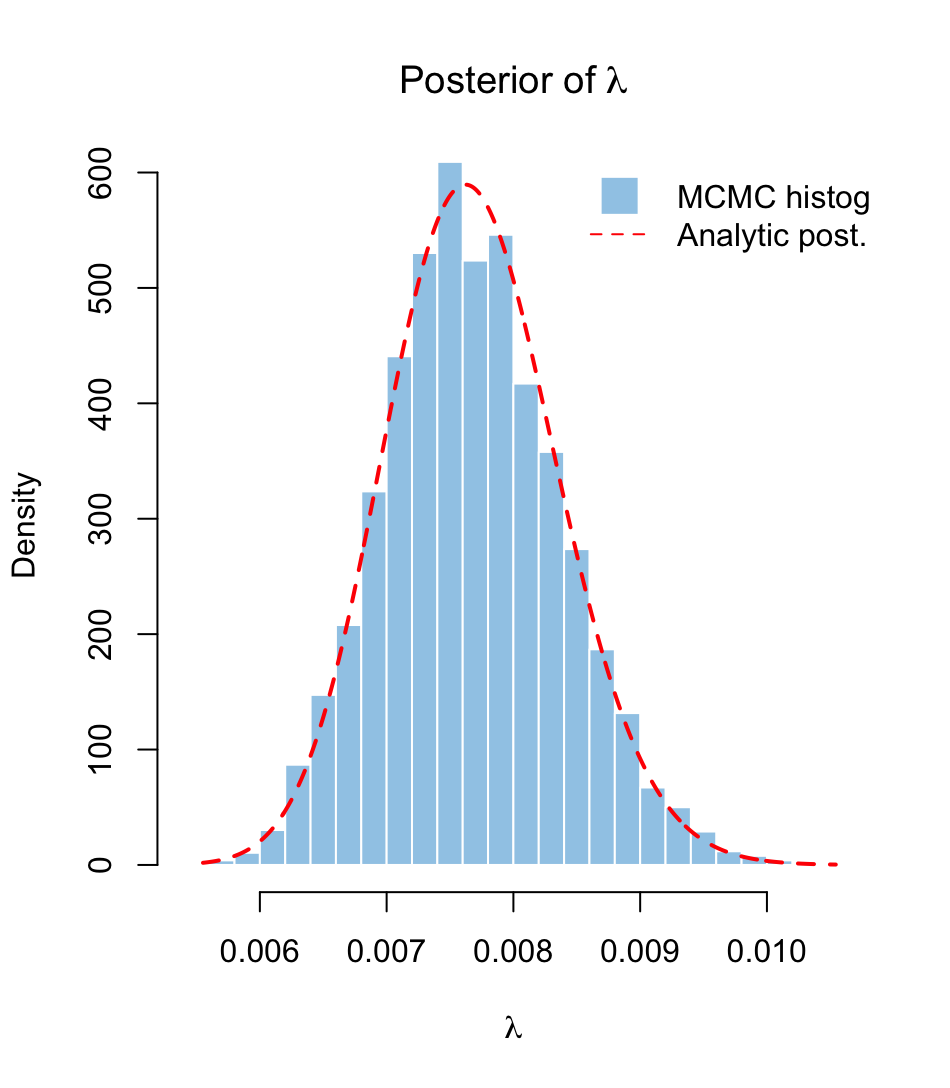
\includegraphics[height=8cm, width=0.5\textwidth]{MSc_Statistics_Research_Report_paper/images/直方图.png}
    \caption{Posterior distribution of $\lambda$ from MCMC samples (histogram) and analytic Gamma posterior (red curve)}
    \label{fig:exp veteran}
\end{figure}


%%%%%%%%%%%%%%%%%%%%%%%%%%%%%%%%
%%%%%%%%%%%%%%%%%%%%%%%%%%%%%
%%%%这后面说的是后验预测
After obtaining the posterior distribution of model parameters $p(\theta \mid D)$, we are often interested in making predictions about future observations. This leads naturally to the posterior predictive distribution, defined as
\begin{equation}
    p(\tilde{y} \mid D) = \int p(\tilde{y} \mid \theta)\, p(\theta \mid D)\, d\theta
    \label{eq:18}
\end{equation}
where $\tilde{y}$ is a new (unseen) observation, $\theta$ denotes the model parameters, and $D$ is the observed dataset. In practice, this integral is often intractable and is therefore approximated using Monte Carlo methods. Specifically, we draw samples $\theta^{(1)}, \theta^{(2)}, \dots, \theta^{(M)}$ from the posterior $p(\theta \mid D)$, and estimate the posterior predictive distribution as
\begin{equation}
p(\tilde{y} \mid D) \approx \frac{1}{M} \sum_{m=1}^{M} p(\tilde{y} \mid \theta^{(m)}).
\end{equation}

\subsection{Model Checking}\label{sec:model checking}
\begin{figure}[H]
\centering
\resizebox{0.52\linewidth}{!}{
\begin{tikzpicture}[
 scale=0.50,
  every node/.style={transform shape}, 
  node distance=11mm,
  box/.style      ={rectangle, draw, rounded corners, align=center,
                    minimum width=44mm, minimum height=9mm},
  decision/.style ={diamond, aspect=2.2, draw, align=center, inner sep=1.4pt},
  ->, >=Latex
]

%--- Main process node ------------------------------------------------------
\node[box]      (model)   {\textbf{Define/Revise a model}};

\node[box]      (checking1)  [below=of model] {\textbf{Model checking} \\
(Simulate with $\lambda_0$; fit model; recover $\lambda_0$?)};

\node[decision] (pass1)   [below=10mm of checking1] {\textbf{Plausible?}};

\node[box]      (fit)     [below=of pass1]  {\textbf{Fit to real data}\\
(Compute posterior)};

\node[box]      (gen)     [below=of fit]    {\textbf{Posterior predictive model checking}\\
(Generate fake data from Posterior)\\
(Compare fake vs real)};

\node[decision] (pass2)   [below=of gen] {\textbf{Adequate?}};

\node[box]     (report)  [below=of pass2] {\textbf{Report/Interpret}};

%--- 连线 ------------------------------------------------------------
\draw (model)   -- (checking1)
      (checking1)  -- (pass1)
      (pass1)   -- node[right]{Yes}(fit)
      (fit)     -- (gen)
      (gen) -- (pass2)
      (pass2) -- node[right]{Yes}(report);

%--- Loopback ------------------------------------
\draw[->] (pass1.west) -- ++(-30mm,0) |- (model.west) node[pos=0.23, left]{No};
%\draw[->] (pass1.west) to[out=180,in=180,looseness=1.3] node[left]{No} (model.west);
\draw[->] (pass2.east) -- ++ (30mm,0 )|- (model.east) node[pos=0.23,right]{No};
\end{tikzpicture}}
\caption{General Bayesian workflow}
\end{figure}

\begin{tcolorbox}[
  title  = Algorithm 1: Simulating a Fake Survival Dataset (e.g.Posterior predictive model checking),
   fonttitle  = \small, 
  colback = white,
  colframe=black]
\textbf{Input}\\
\quad$\bullet$ posterior samples $\{\lambda^{(s)}\}$ \hfill (obtained by fitting real data)\\
\quad$\bullet$ sample size $n$ \hfill (same size as the real data set)\\
\quad$\bullet$ start‑time range $[a,0]$ with $a<0$ \\[6pt]
\textbf{Algorithm}\par
\begin{enumerate}
  \item Choose a single $\lambda^\ast$ from posterior samples \hfill (e.g.\ posterior mean)
  \item For $i = 1,\dots,n$
        \begin{enumerate}
          \item[] \hspace*{-10pt}%
          \begin{minipage}[t]{\linewidth}
          \begin{enumerate}
            \item Draw latent duration: $y_i \sim \operatorname{Exp}(\lambda^\ast)$
            \item Draw start time: $T_i \sim \operatorname{Uniform}(a,0)$
            \item Compute leaving time: $t_i = T_i + y_i$
            \item Observed pair $(\text{time}_i,\text{event}_i)$ \[\begin{aligned}
\text{if } \quad t_i &< 0: &&&\text{(event occurred before now)}\\
  &&\quad  \text{event}_i=1, &&\text{(uncensored)}\\ 
  &&\quad \text{time}_i=y_i
   &\quad \\
&\text{else}: &&&\text{(event in the future)}\\
   &&\quad \text{event}_i=0, &&\text{(right censored)}\\ 
   &&\quad \text{time}_i=-T_i &&\text{(time already spent)}
   &\quad 
\end{aligned}\]
          \end{enumerate}
          \end{minipage}
        \end{enumerate}
  \item Combine $(\text{time}_i,\text{event}_i)$ into a fake data set of size $n$.
\end{enumerate}
\label{fake data}
\end{tcolorbox}

\subsubsection{Model Checking via ECDF under Independent Censoring}
In model checking, to compare the overall distributional shapes of the real data and the simulated data, we use the empirical cumulative distribution function (ECDF) rather than histograms. Unlike histograms, ECDFs do not depend on subjective choices of bin widths and break points, thereby avoiding visual biases. Moreover, an ECDF is a monotone right-continuous step function defined on $[0,\infty)$, which stably displays differences between samples over the entire time axis. Importantly, ECDFs can be plugged directly into distance statistics such as the Kolmogorov–Smirnov or Cramér–von Mises metrics, facilitating quantitative assessment of model fit.

In survival data, the observed duration is determined jointly by the latent event time $T\ge 0$ and the censoring time $C\ge 0$. The observed quantity is
$$
Y=\min(T,C),\qquad \delta=\mathbf 1\{T\le C\}.
$$
That is, we observe the event time only when it is uncensored; otherwise, we observe the censoring time. Consequently, we split the data into two subsamples—an “event subsample’’ with $\delta=1$ and a “censored subsample’’ with $\delta=0$—and compute ECDFs for each subsample separately.

Under independent (non-informative) censoring, i.e., $T\perp C$, the two subsamples may be viewed as arising from two conditional distributions
\begin{itemize}
    \item for the event subsample ($\delta=1$), the observed values $Y=T$ follow the conditional distribution $T\mid(T\le C)$;
    \item for the censored subsample ($\delta=0$), the observed values $Y=C$ follow the conditional distribution $C\mid(C<T)$.
\end{itemize}
Let the event-subsample size be $n_1=\sum_i \delta_i$ and the censored-subsample size be $n_0=\sum_i (1-\delta_i)$. The corresponding empirical distribution functions are
\begin{equation}
    \widehat H_{\text{event}}(t)
=\frac{1}{n_1}\sum_{i:\,\delta_i=1}\mathbf 1\{Y_i\le t\},\qquad
\widehat H_{\text{cens}}(t)
=\frac{1}{n_0}\sum_{i:\,\delta_i=0}\mathbf 1\{Y_i\le t\},\qquad t\ge 0.
\end{equation}
By the Glivenko–Cantelli theorem (\cite{tucker1959generalization}), as sample sizes grow, these ECDFs converge uniformly to their respective target distribution functions
\begin{align}
\widehat H_{\text{event}}(t) &\xrightarrow{\text{uniformly in } t} H_{\text{event}}(t) := \Pr(T \le t \mid T \le C) \\
\widehat H_{\text{cens}}(t) &\xrightarrow{\text{uniformly in } t} H_{\text{cens}}(t) := \Pr(C \le t \mid C < T)
\end{align}
In summary, by splitting the data into event and censored subsamples and plotting their empirical distribution functions $\widehat H_{\text{event}}$ and $\widehat H_{\text{cens}}$, we can evaluate model fit within a unified framework along both dimensions.



%%%%%%%%%%%%%%%%%%%%%%%%%%%%%%%%%%%%%%%%%%%%%%%
\subsubsection{Choosing and Interpreting the Survey-Length Parameter $A$}

In the posterior predictive model checking of this study, we generate simulated data from the model and compare it with the observed data. This simulation relies on sampling given known quantities; a key quantity is the \textbf{maximum survey duration $A$ }in Algorithm 1 (\ref{fake data}), which is controlled by the user-specified parameter $a$, with the reparameterization $A = -a$, governing the censoring mechanism in the simulated data. In other words, $A$ sets the observation window in simulation and thereby affects both the censoring rate and the distribution of event times.

This quantity is not a parameter to be estimated by the model; it is an external input required to generate fake data. Although it may appear auxiliary, it is tightly coupled with model checking—different choices of $A$ change the censoring structure of the simulated data and therefore influence the credibility of posterior predictive results.

Does the observed data carry information about $A$? Yes. In any survival dataset, the “shadow” of the survey window is reflected in the censoring proportion and the shape of the observed durations. If the survey is short (small $A$), many subjects are censored before the event occurs, leading to a high right-censoring rate and “compressed” event times. Conversely, with a long survey (large $A$), more events are observed, censoring decreases, and event times spread out.

This can be seen in Figure~\ref{fig:离职数据分开的直方图} (histograms of event and censored durations in the employee turnover data). The number of events and censors is roughly balanced, suggesting that the survey was long enough to capture about half of the departures. Since the maximum observed duration exceeds 170 months, it is reasonable to infer that the underlying survey duration $A$ should be at least greater than 170; this directly informs how the censoring mechanism should be set in simulation.
\begin{figure}[H]
    \centering
    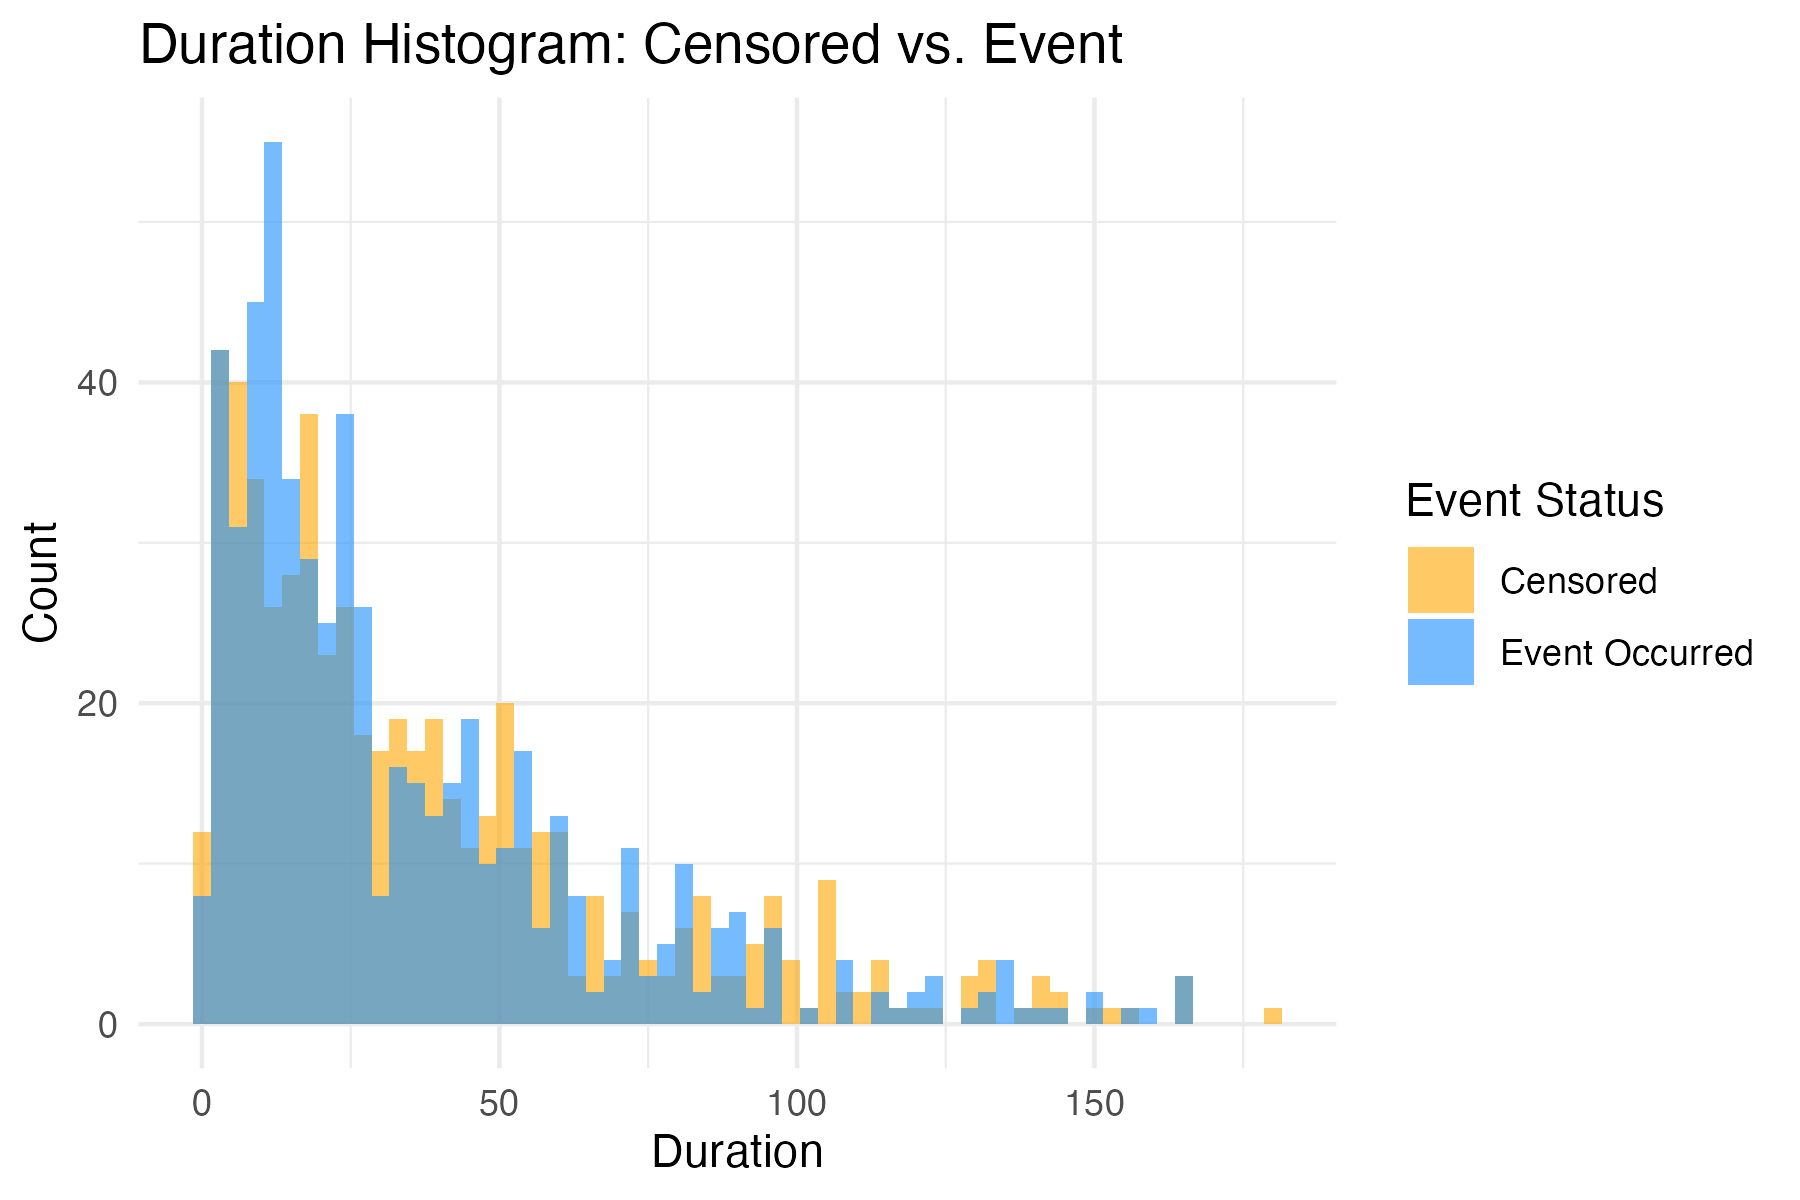
\includegraphics[height=5.5cm, width=0.6\textwidth]{images/separate_hist.png}
    \caption{Histograms of censored and event durations in the employee turnover data}
    \label{fig:离职数据分开的直方图}
\end{figure}
To further support this point, we simulate under two settings, $A = 30$ and $A = 1000$, and plot the empirical cumulative distribution functions (ECDFs) for both the event subsample ($\delta = 1$) and the censored subsample ($\delta = 0$), along with the histograms of simulated durations.
\begin{itemize}
    \item $A = 30$ (Figure~\ref{fig:ppc-A30}). Compared to the real-data histogram (Figure~\ref{fig:离职数据分开的直方图}), the simulated durations in Figure~\ref{fig:fake-hist_a30} are heavily compressed within 0–30 months, indicating that both events and censorings occur unusually early. Correspondingly, the ECDFs for events and censorings (Figure~\ref{fig:ecdf-cens_a30}~\ref{fig:ecdf-event_a30}, red lines) rise too steeply at short durations, deviating noticeably from the observed curves. This mismatch is primarily driven by an unrealistic observation window $A$, rather than a misfit of the event-time distribution (e.g., the parameter $\lambda$) itself.
    \item $A = 1000$ (Figure~\ref{fig:ppc-A1000})
  In contrast, Figure~\ref{fig:fake-hist_a1000} shows a histogram with a much wider and sparser spread of durations, and the ECDF curves (Figure~\ref{fig:ecdf-event_a1000}~\ref{fig:ecdf-cens_a1000}, red lines) align more closely with the observed data. However, when compared to the real-data histogram in Figure~\ref{fig:离职数据分开的直方图}, this setting exceeds any realistic survey length—implying a maximum tenure close to 83 years—which is implausible in practical employment contexts. Thus, although the simulated curves fit better visually, this apparent “match” relies on an unrealistic assumption about $A$, and should not be accepted as a reliable model-checking result.
\end{itemize}
These two examples reinforce a key point: when performing posterior predictive checks, fit quality must be evaluated alongside the realism of the data-generating assumptions in simulation.
\begin{figure}[htbp]
\centering
\begin{subfigure}[t]{0.3\textwidth}
  \centering
  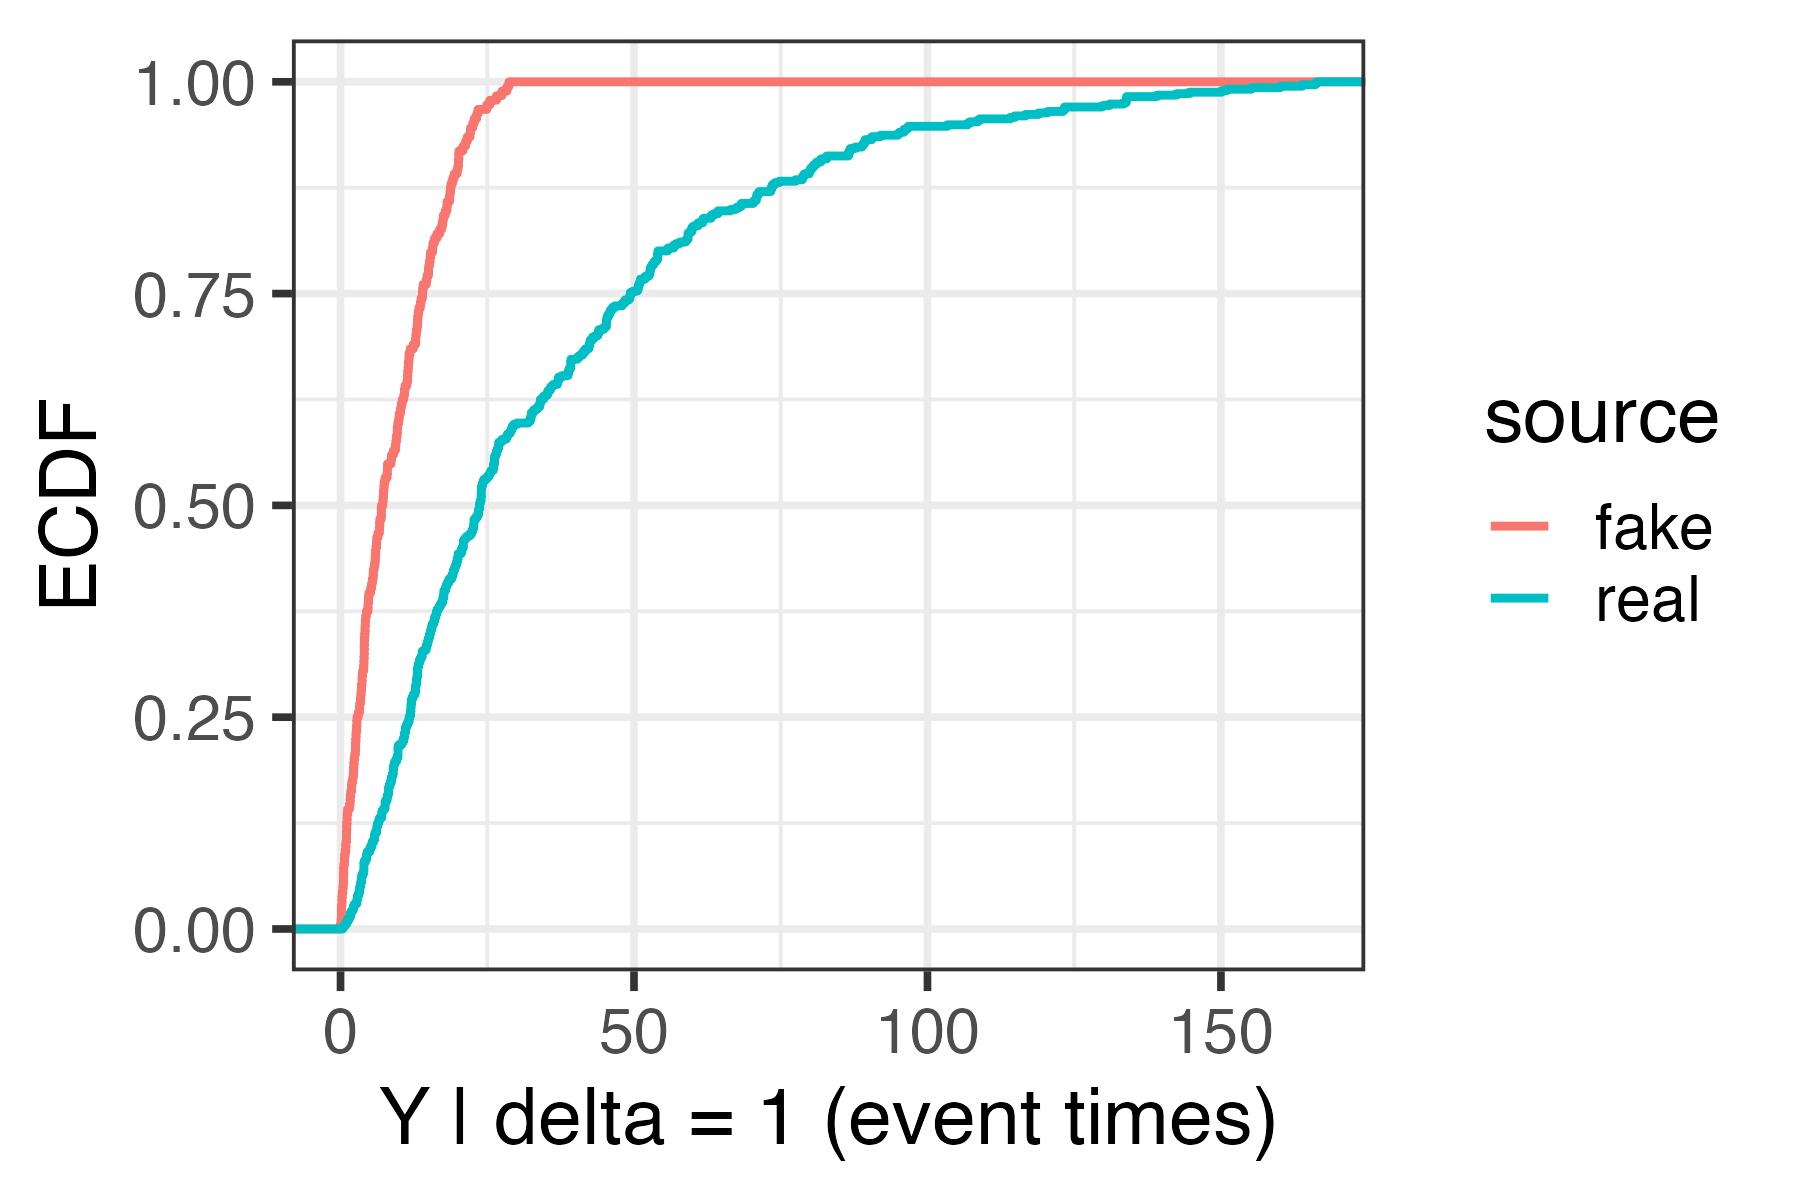
\includegraphics[width=\linewidth]{images/ppc_event_ecdf_A30.png}  % 图1路径
  \caption{ECDF of $Y \mid \delta=1$}
  \label{fig:ecdf-event_a30}
\end{subfigure}\hfill
\begin{subfigure}[t]{0.3\textwidth}
  \centering
  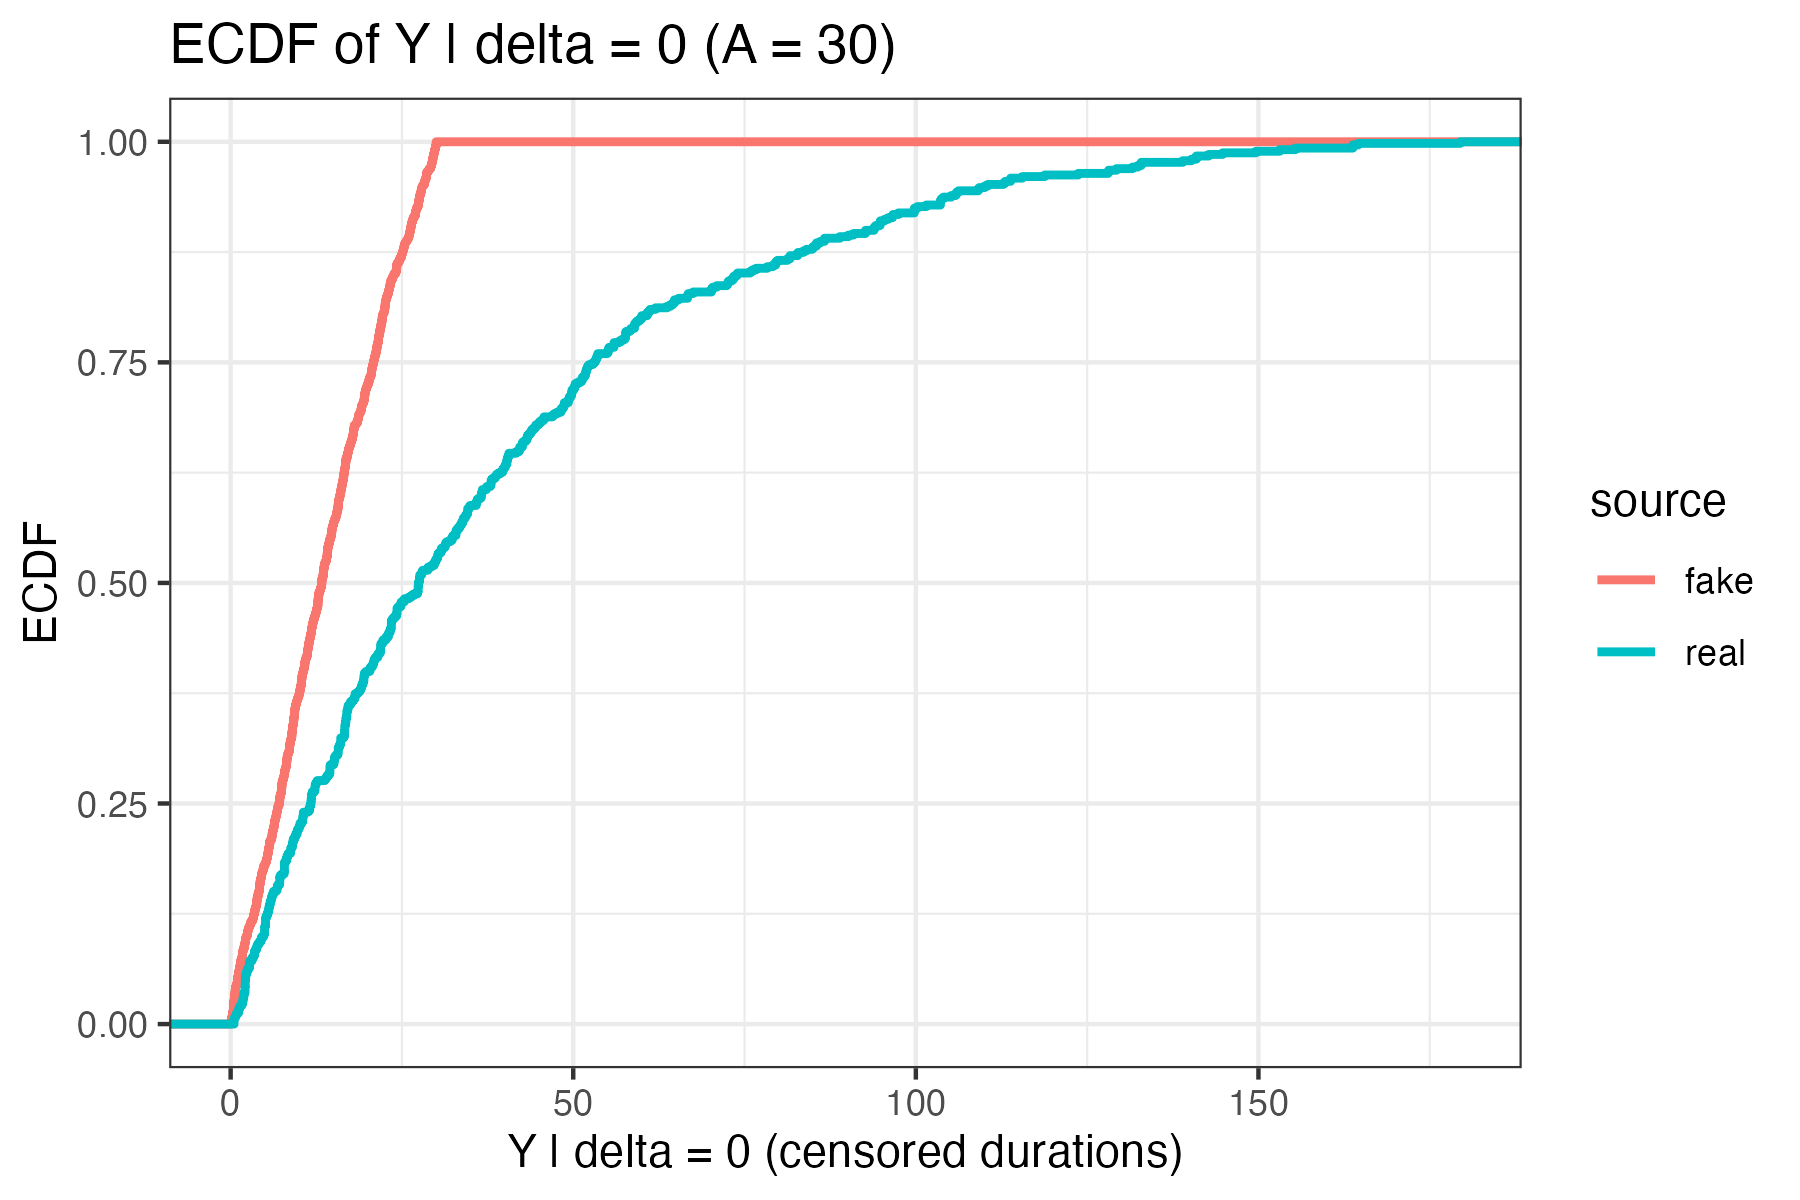
\includegraphics[width=\linewidth]{images/ppc_censored_ecdf_A30.png}   
  \caption{ECDF of $Y \mid \delta=0$}
  \label{fig:ecdf-cens_a30}
\end{subfigure}\hfill
\begin{subfigure}[t]{0.37\textwidth}
  \centering
  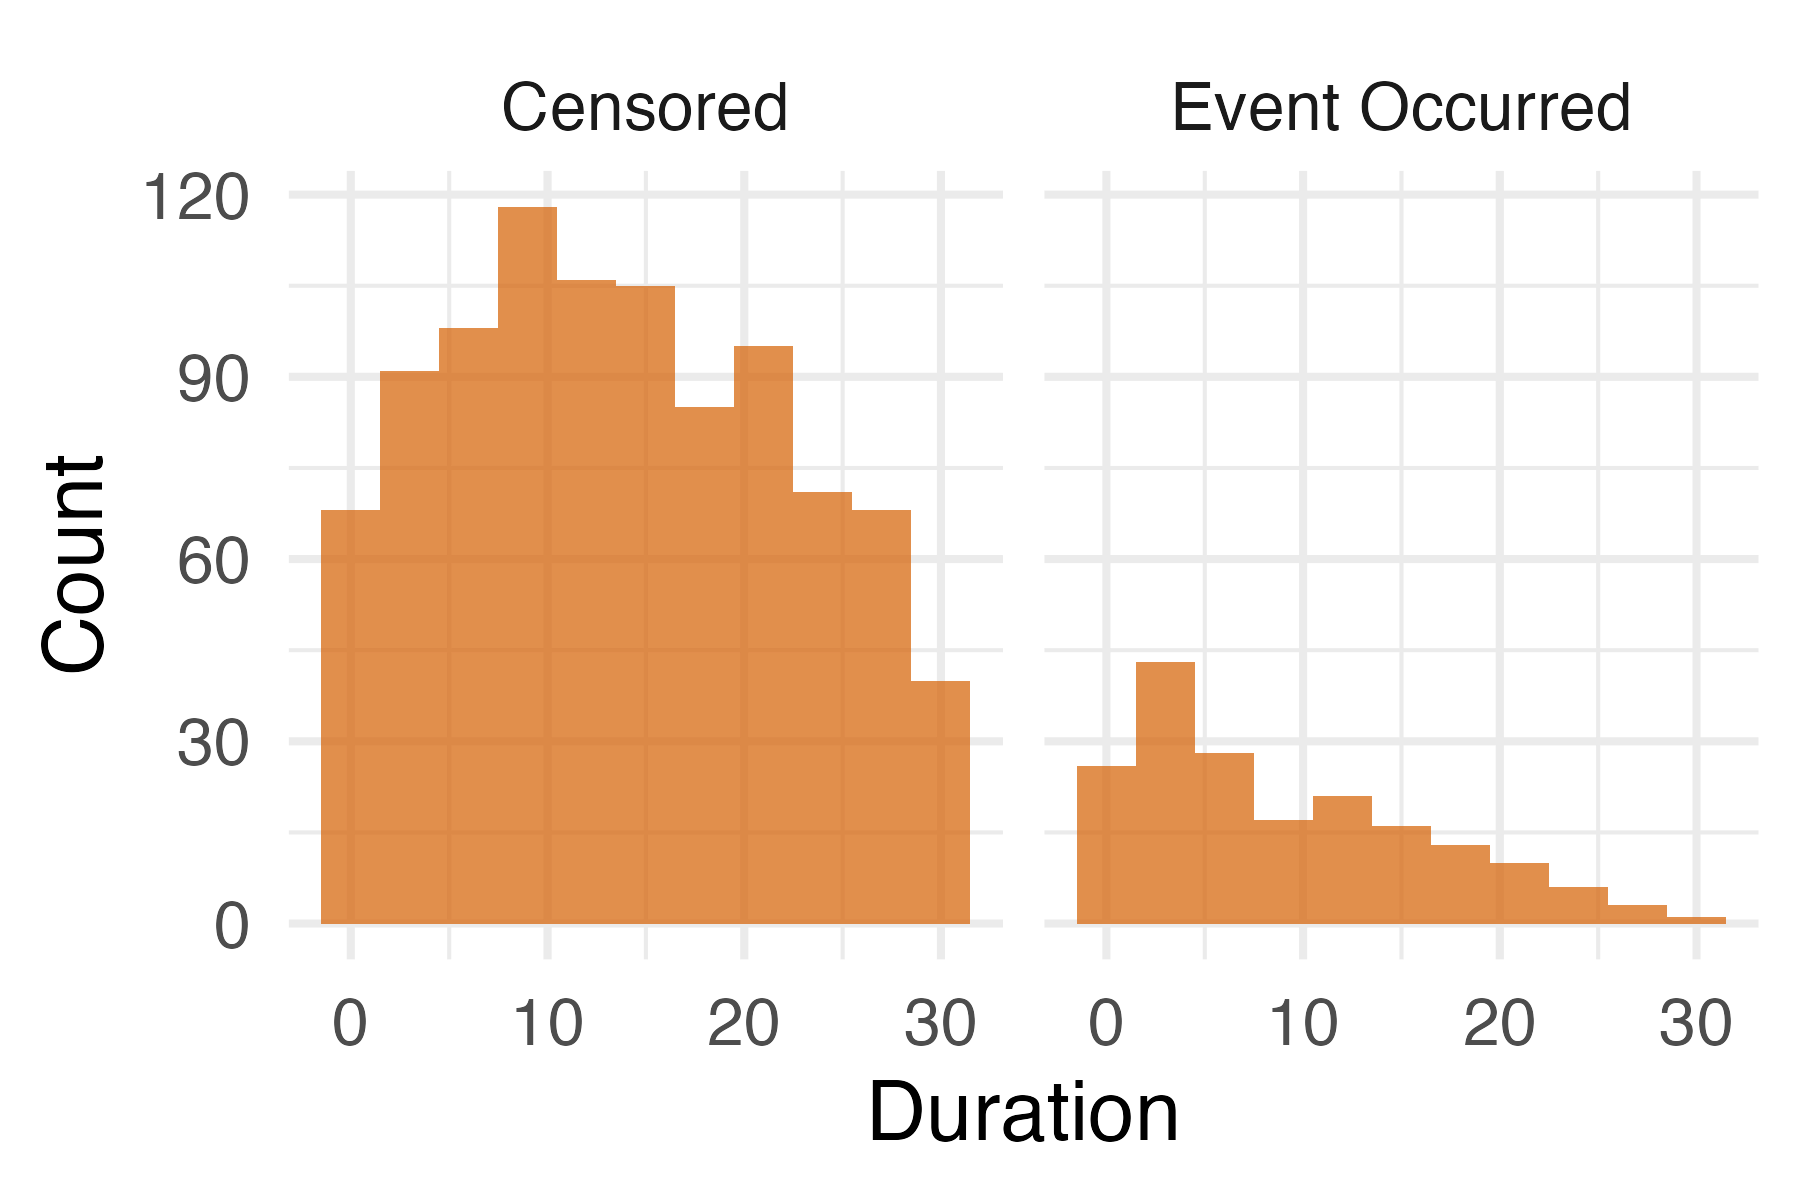
\includegraphics[width=\linewidth]{images/fake_duration_hist_a30.png}   % 图3路径
  \caption{Fake-data histogram}
  \label{fig:fake-hist_a30}
\end{subfigure}
\caption{Posterior predictive checking ($A=30$).}
\label{fig:ppc-A30}
\end{figure}
%%%%%%%%%%%%%%%%%%%%%%
\begin{figure}[htbp]
\centering
\begin{subfigure}[t]{0.3\textwidth}
  \centering
  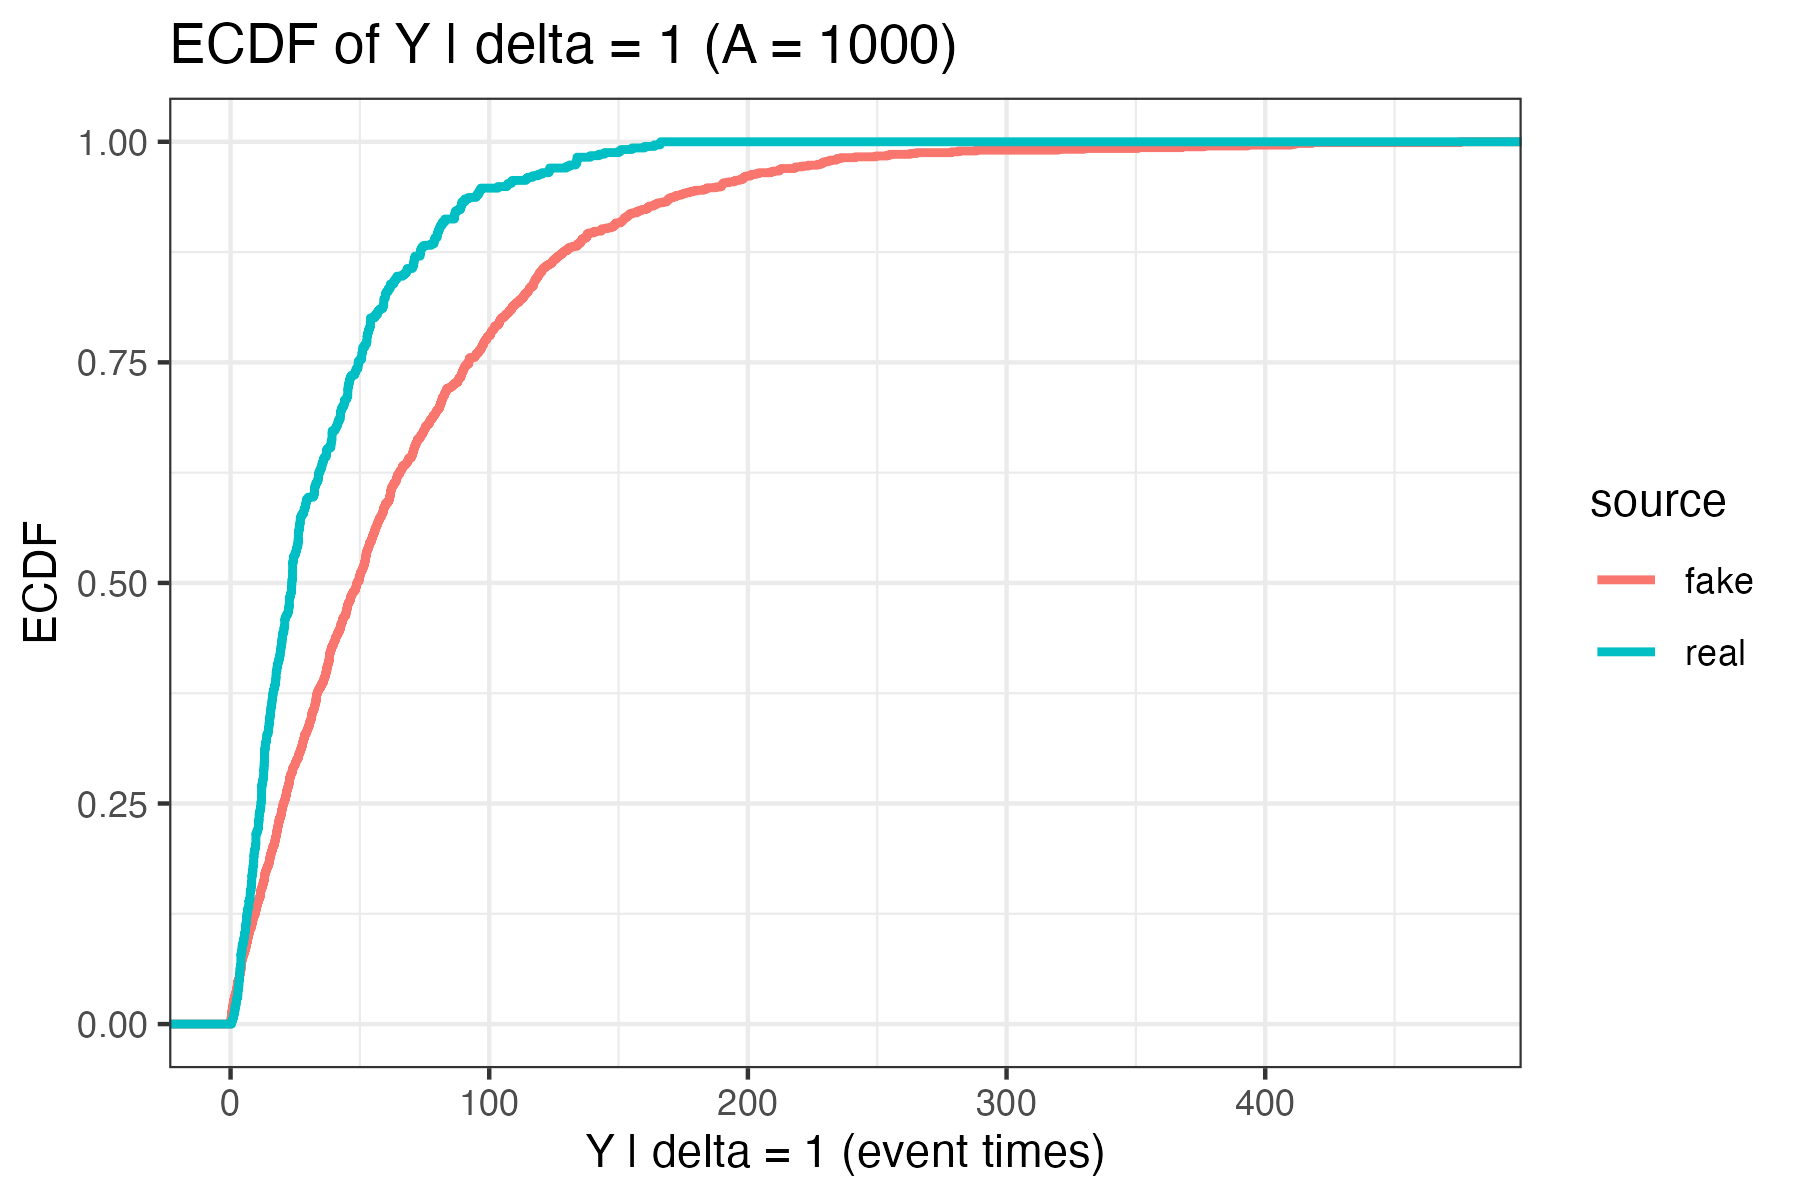
\includegraphics[width=\linewidth]{images/ppc_event_ecdf_A1000.png}  % 图1路径
  \caption{ECDF of $Y \mid \delta=1$}
  \label{fig:ecdf-event_a1000}
\end{subfigure}\hfill
\begin{subfigure}[t]{0.3\textwidth}
  \centering
  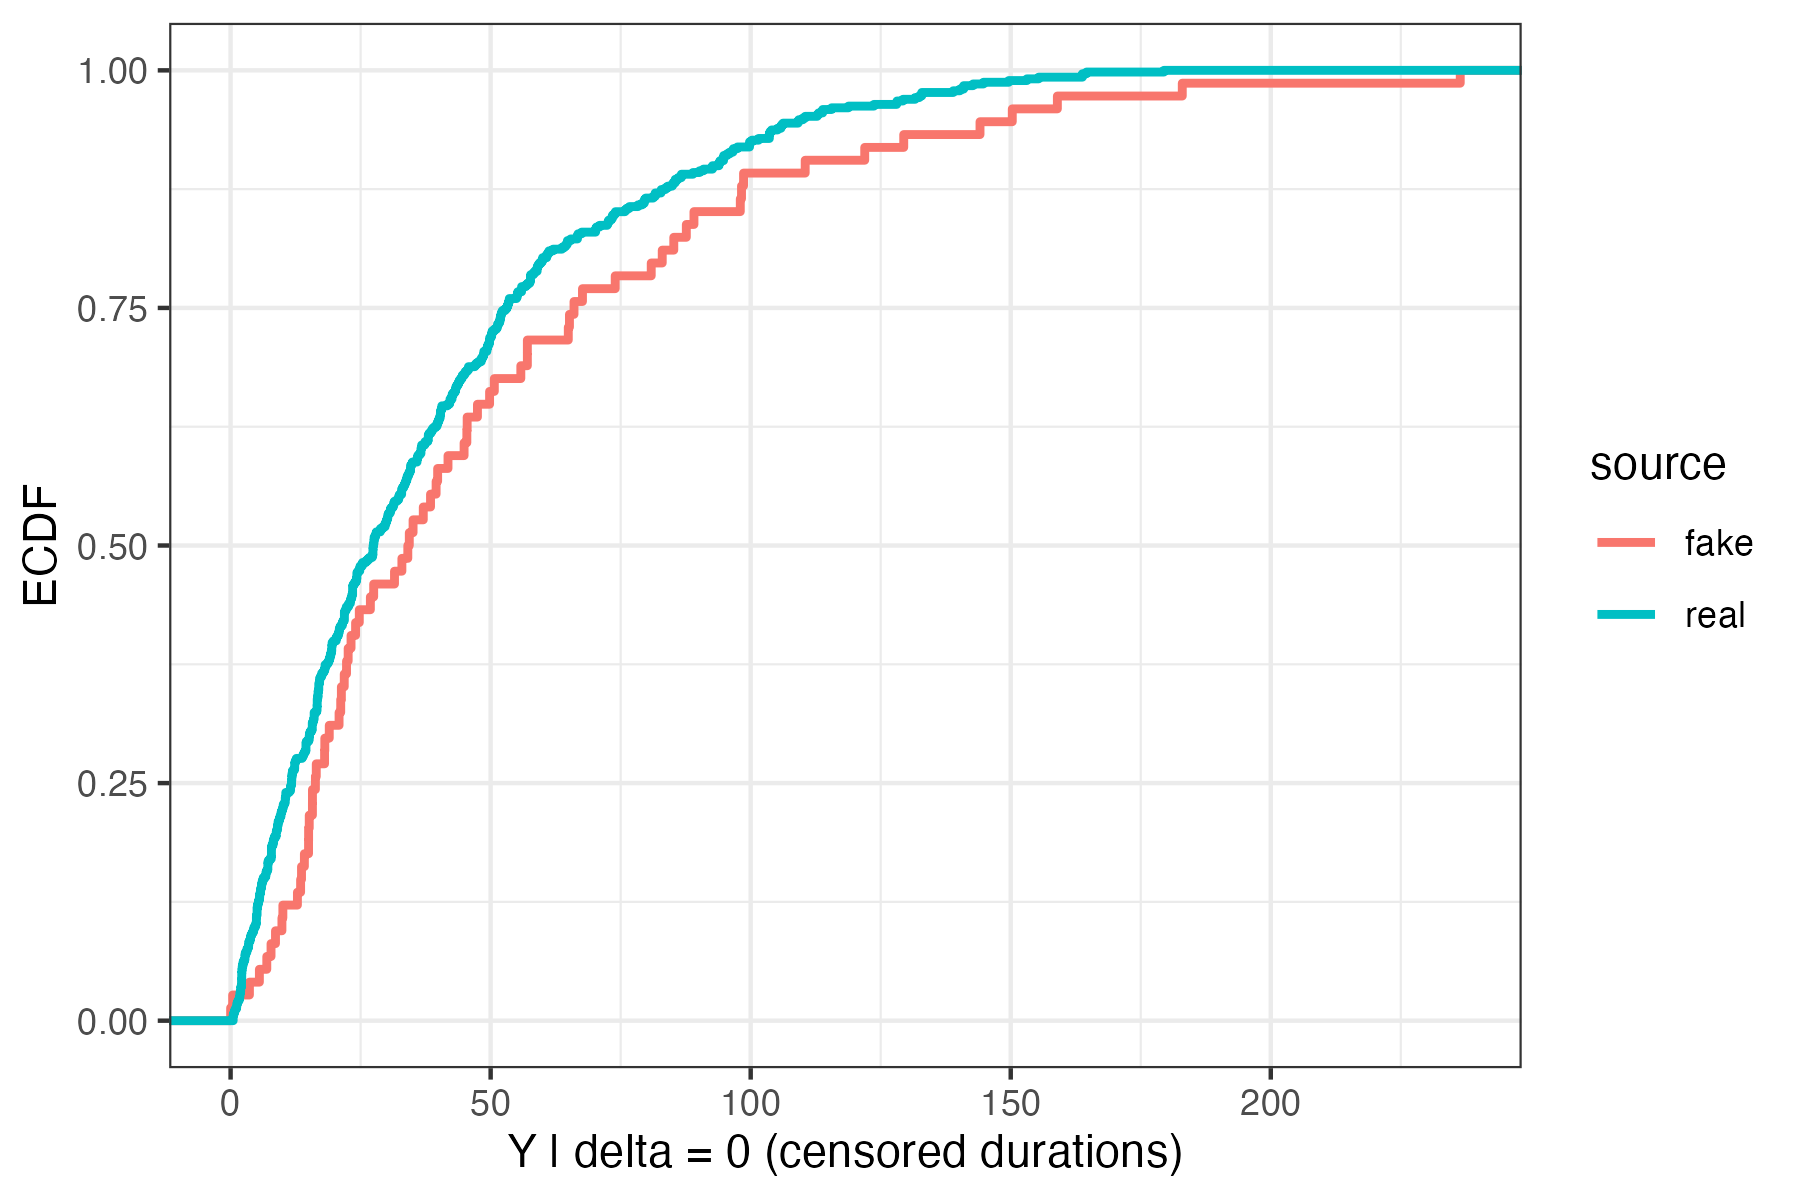
\includegraphics[width=\linewidth]{images/ppc_censored_ecdf_A1000.png} 
  \caption{ECDF of $Y \mid \delta=0$}
  \label{fig:ecdf-cens_a1000}
\end{subfigure}\hfill
\begin{subfigure}[t]{0.37\textwidth}
  \centering
  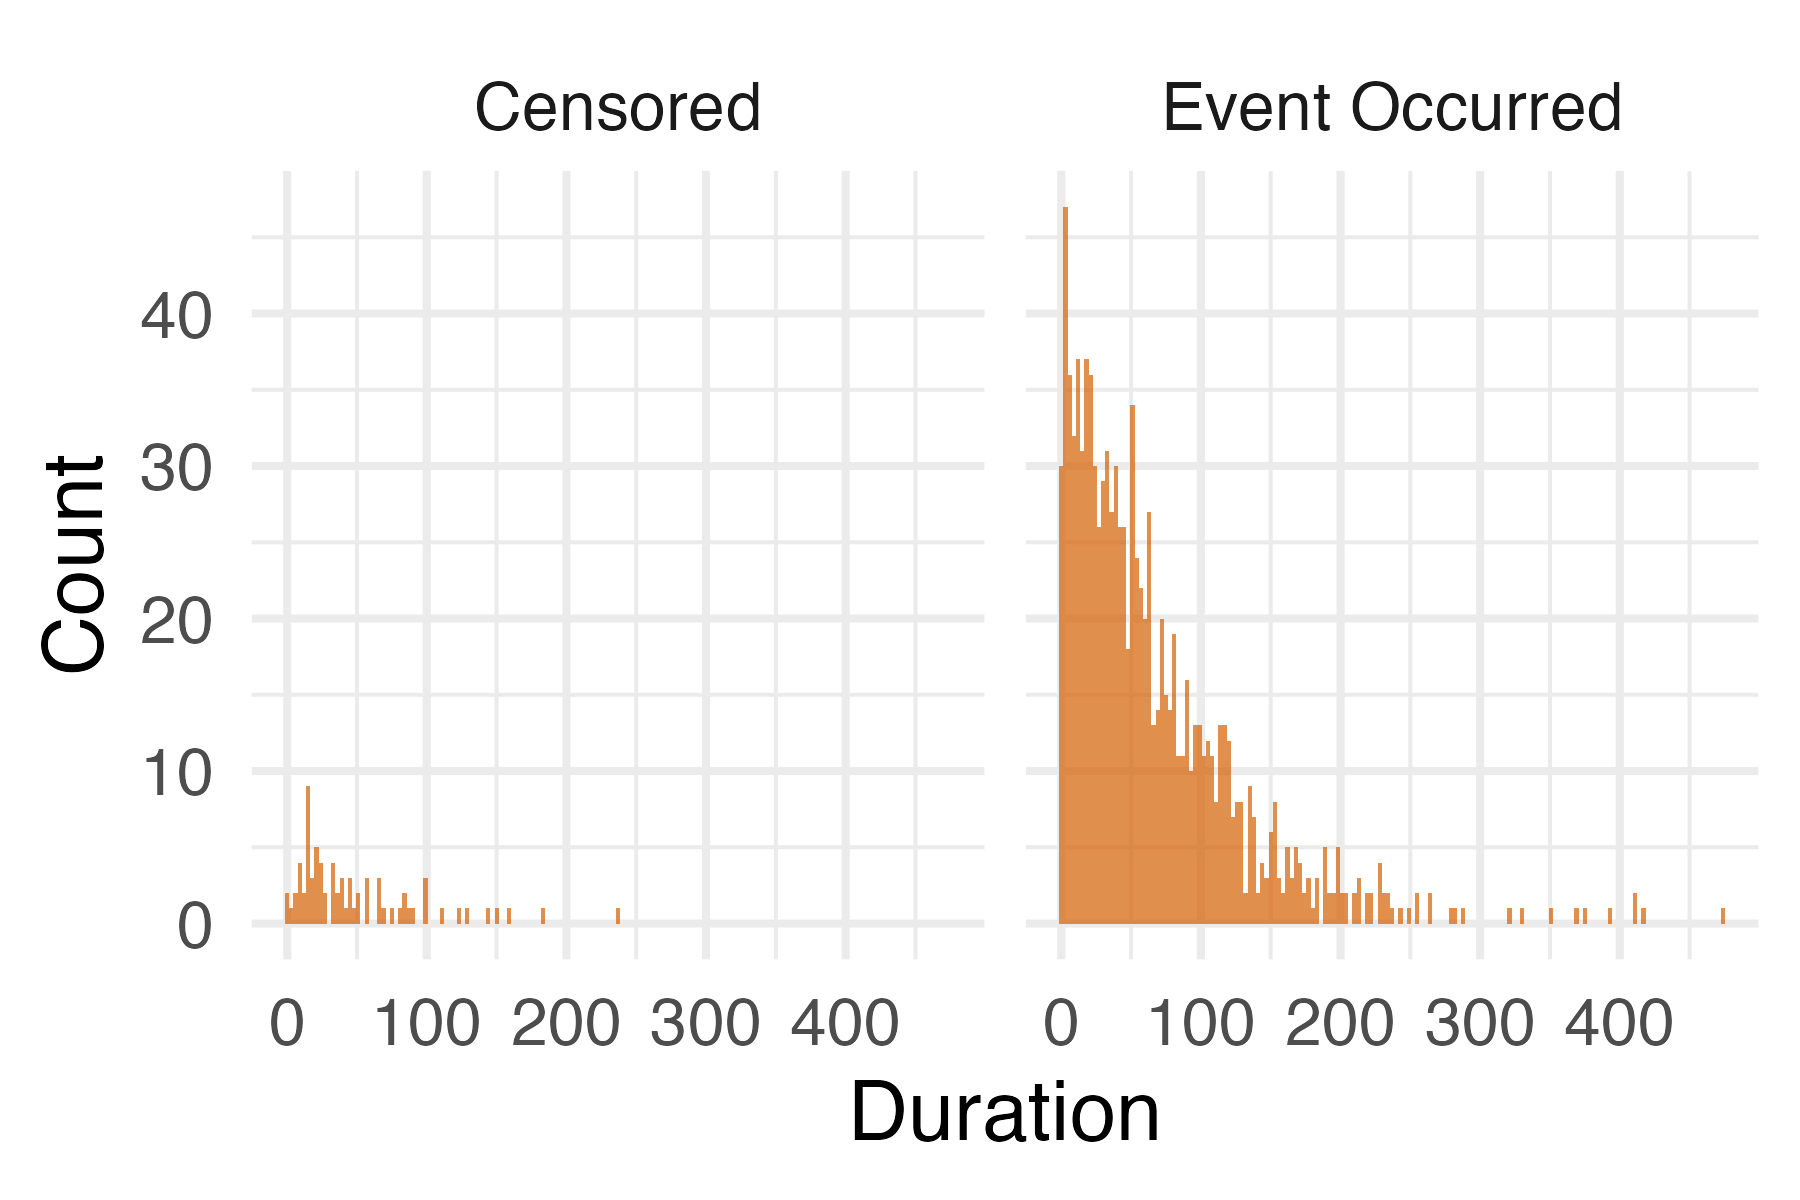
\includegraphics[width=\linewidth]{images/fake_duration_hist_a1000.png}   % 图3路径
  \caption{Fake-data histogram}
  \label{fig:fake-hist_a1000}
\end{subfigure}
\caption{Posterior predictive checking ($A=1000$).}
\label{fig:ppc-A1000}
\end{figure}


%\subsection{Posterior predictive CDF}
%\input{MSc_Statistics_Research_Report_paper/section/Methods_subsection/posterior predictive cdf }

























